\section{Conceito}
\label{sec:conceito}

Para apresentar a teoria dos leilões como uma construção lógica clara --- sem depender de formalismo excessivo ---, definimos explicitamente cada termo antes de utilizá-lo no passo seguinte.

\subsection{Leilões como Jogos Bayesianos}
\label{subsec:jogos_bayesianos}

\begin{definicao}[Jogo de Informação Completa]
\label{def:info_completa}
É um jogo em que todos os jogadores conhecem perfeitamente quem são os participantes, quais ações cada um pode tomar e \textbf{quanto cada jogador ganha (\textit{payoff}) em qualquer combinação de ações}. Não há segredo sobre os objetivos, custos ou avaliações dos adversários \cite{gibbons1992}.
\end{definicao}

No \textit{Dilema dos Prisioneiros}, por exemplo, o Prisioneiro~A sabe exatamente quantos anos de pena o Prisioneiro~B recebe em cada célula da matriz. Porém, em um leilão real, a informação completa não existe: quem disputa um imóvel ou uma concessão pública sabe quanto o bem vale para si, mas \textbf{não sabe quanto ele vale para o seu concorrente}. Isso nos leva à segunda definição:

\begin{definicao}[Jogo de Informação Incompleta / Jogo Bayesiano]
\label{def:jogo_bayesiano}
É um jogo no qual pelo menos um jogador desconhece a função de \textit{payoff} (o ganho líquido) de outro jogador, porque esse ganho depende de informações privadas que só o outro jogador conhece \cite{harsanyi1967,gibbons1992}.
\end{definicao}

Até a década de 1960, os economistas acreditavam ser impossível aplicar o Equilíbrio de Nash a jogos de informação incompleta: para saber minha melhor jogada, preciso prever a jogada do adversário, que depende do \textit{payoff} secreto dele; logo, eu teria que estimar o que acho do \textit{payoff} dele, e o que ele acha que eu acho do \textit{payoff} dele, gerando uma regressão infinita de crenças. \cite{vickrey1961} e \cite{harsanyi1967} resolveram esse impasse por meio da \textbf{Transformação de Harsanyi}, baseada nos conceitos de \textbf{Tipo Privado} e \textbf{\textit{Prior} Comum}:

\begin{definicao}[Tipo Privado ($\theta_i$)]
\label{def:tipo_privado}
É o pedaço de informação secreta que pertence exclusivamente ao jogador $i$ e que determina o seu \textit{payoff}. Nos leilões, o \textbf{tipo} de um comprador nada mais é do que a sua informação privada sobre o valor do objeto (o máximo que ele estaria disposto a pagar, ou a estimativa técnica que a sua equipe fez sobre o bem).
\end{definicao}

Por exemplo, se duas construtoras disputam uma licitação para erguer uma ponte, e a Construtora~1 (com máquinas novas) faz a obra por R\$\,80 milhões enquanto a Construtora~2 (com máquinas antigas) gasta R\$\,95 milhões, esse custo interno secreto é o \textbf{Tipo ($\theta_i$)} de cada uma: cada empresa vê a sua própria planilha, mas não vê a da concorrente. Como então tomar uma decisão racional?

\begin{definicao}[Distribuição de Crenças a Priori / \textit{Prior} Comum $F$]
\label{def:prior_comum}
É a distribuição conjunta de probabilidade $F(\theta_1, \theta_2, \dots, \theta_n)$ segundo a qual a ``Natureza'' sorteia os \textbf{Tipos} de todos os jogadores antes de o jogo começar, sendo essa regra estatística de sorteio conhecida por todos os participantes \cite{harsanyi1967,gibbons1992}.
\end{definicao}

Vale esclarecer três pontos sobre o \textit{Prior} Comum $F$:
\begin{enumerate}[label=\arabic*.]
    \item \textbf{Origem do termo \textit{Prior}:} Vem da Estatística Bayesiana (\textit{a priori}, em oposição a \textit{a posteriori}). Harsanyi propôs imaginar que o jogo começa um passo antes, com um jogador fictício chamado \textbf{Natureza}: no estágio inicial (\textit{ex ante}), a Natureza gira uma roleta probabilística $F$ e sorteia um cartão secreto com o Tipo $\theta_i$ para cada jogador $i$ (\textit{Prior}); em seguida (\textit{estágio interim}), cada jogador espia apenas o seu próprio cartão $\theta_i$ e atualiza suas probabilidades usando a Regra de Bayes.
    \item \textbf{Por que se chama ``Comum''?} ``Prior Comum'' \textbf{não} significa que todos os jogadores são sorteados da mesma curva estatística. Vem de \textit{Conhecimento Comum} (\textit{Common Knowledge}): todos os jogadores da mesa conhecem e concordam sobre quais são as regras da roleta da Natureza ($F$).
    \item \textbf{Simetria, Assimetria e Correlação:} Dentro da lei geral $F(\theta_1, \dots, \theta_n)$, ocorrem três casos práticos: (a) \textit{Distribuição Universal / Jogadores Simétricos ($F_1 = \dots = F_n$)}, como dois estudantes disputando um ingresso com valores sorteados entre R\$\,0 e R\$\,100 (caso da Seção~\ref{sec:modelo_resolvido}); (b) \textit{Distribuição Particular / Jogadores Assimétricos ($F_1 \neq F_2$)}, como num leilão do 5G em que o valor de uma grande operadora sai de $[500, 1000]$ milhões ($F_1$) e o de uma provedora regional sai de $[100, 400]$ milhões ($F_2$), sendo ambas as curvas conhecidas por todos; e (c) \textit{Tipos Correlacionados}, como no pôquer, em que o baralho de 52 cartas é o mesmo \textit{Prior} inicial para todos, mas após cada jogador olhar suas cartas ($\theta_i$), cada um passa a ter uma distribuição condicional (\textit{posterior} $F(\theta_{-i} \mid \theta_i)$) diferente.
\end{enumerate}

Na notação da Teoria dos Jogos, o subscrito \textbf{``$-i$''} (``todos exceto $i$'') indica o vetor dos concorrentes de $i$: $\theta_{-i} = (\theta_1, \dots, \theta_{i-1}, \theta_{i+1}, \dots, \theta_n)$ e $b_{-i} = (b_1, \dots, b_{i-1}, b_{i+1}, \dots, b_n)$ (com 2 jogadores, $\theta_{-1} = \theta_2$ e $b_{-1} = b_2$). Com isso, definimos estratégia e equilíbrio:

\begin{definicao}[Estratégia em um Jogo Bayesiano ($b_i(\theta_i)$)]
\label{def:estrategia_bayesiana}
Em um jogo bayesiano, uma estratégia \textbf{não é uma única ação isolada}, mas sim um \textbf{plano completo (uma função matemática)} que especifica qual ação (lance) o jogador $i$ escolherá \textbf{para cada Tipo $\theta_i$ que a Natureza possa ter sorteado para ele} \cite{gibbons1992}.
\end{definicao}

A estratégia precisa ser uma função porque o Jogador~1 (que tirou, digamos, $v_1 = 80$) não sabe qual valor $v_2$ o Jogador~2 tirou hoje ($10$, $50$ ou $90$); logo, ele só consegue calcular a probabilidade de vencer se souber a \textbf{regra (função)} $b_2(v_2)$ que o Jogador~2 usa para converter qualquer valor $v_2$ em um lance (por exemplo, $b_2(v_2) = 0{,}5\,v_2$).

\begin{definicao}[Equilíbrio de Nash Bayesiano --- ENB]
\label{def:enb}
É um perfil de funções de estratégia ($b_1^*(\theta_1),$ $\dots,$ $b_n^*(\theta_n)$) --- uma regra de lance para cada jogador --- tal que, para todo jogador $i$ e para todo Tipo possível $\theta_i$ desse jogador, o lance $b_i^*(\theta_i)$ maximiza o \textbf{ganho médio esperado} de $i$ (calculado sobre a distribuição de tipos dos adversários $F(\theta_{-i} \mid \theta_i)$), dado que todos os outros jogadores estão usando as funções de lance $b_{-i}^*(\theta_{-i})$.
\end{definicao}

Destacamos duas propriedades importantes do ENB: (i) a função $b_i^*(\theta_i)$ atinge o ganho máximo para \textit{qualquer tipo próprio $\theta_i$} (pois o jogador já conhece seu próprio tipo ao dar o lance), mas apenas \textit{na média esperada (\textit{interim})} sobre os tipos dos outros $\theta_{-i}$ (no 1º preço, $b^*(v_i) = v_i/2$ é ótimo em média antes de abrir os envelopes; já no 2º preço de Vickrey, a estratégia sincera $b^*(v_i) = v_i$ é ainda mais forte, pois é ótima para \textit{qualquer combinação realizada $(v_1, v_2)$}, constituindo um Equilíbrio em Estratégias Dominantes / \textit{Ex Post}); e (ii) no ENB, todos conhecem a \textbf{função (fórmula)} dos adversários (como uma ``calculadora de vidro transparente'' programada para dividir por 2), mas o segredo está no \textbf{número $v_j$} que cada adversário digitou na calculadora hoje.

% =============================================================================
\subsection{Valores Privados e Valores Comuns}
\label{subsec:valores_privados_comuns}

\begin{definicao}[Valoração ($v_i$) e Excedente / \textit{Payoff} ($u_i$)]
\label{def:valoracao_payoff}
A \textbf{Valoração ($v_i$)} é o valor monetário máximo que o objeto leiloado tem para o jogador $i$ (sua disposição máxima a pagar). Se o jogador $i$ vence o leilão e paga um preço $p$, o seu ganho líquido (\textbf{Excedente do Comprador} ou \textbf{\textit{Payoff}}) é $u_i = v_i - p$. Se perde o leilão e não paga nada, seu \textit{payoff} é $u_i = 0$.
\end{definicao}

Na literatura de leilões, há dois ambientes clássicos que relacionam a Valoração $v_i$ com o Tipo $\theta_i$ \cite[p.~13--14]{klemperer2004}:

\begin{definicao}[Modelo de Valores Privados Independentes --- IPV (\textit{Independent Private Values})]
\label{def:ipv}
É o ambiente de leilão em que: (1) \textbf{Valor Privado ($v_i = \theta_i$):} cada jogador $i$ conhece com $100\%$ de certeza qual é a sua própria Valoração $v_i$ antes do leilão começar; mesmo que ele descobrisse o Tipo dos concorrentes, isso \textbf{não mudaria em um centavo} o quanto o objeto vale para ele; e (2) \textbf{Independência Estatística:} o valor $v_i$ de um jogador foi sorteado de forma independente do valor $v_j$ dos outros jogadores.
\end{definicao}

Um exemplo de Valor Privado é o leilão de uma camisa autografada do time de coração (para uso próprio, sem revenda): se ela vale R\$\,500 para você, descobrir que seu vizinho daria apenas R\$\,20 porque torce para outro time não altera o fato de que ela continua valendo R\$\,500 para você.

\begin{definicao}[Modelo de Valor Comum Puro --- CV (\textit{Common Value})]
\label{def:cv}
É o ambiente de leilão em que o objeto tem \textbf{exatamente o mesmo valor final objetivo $V$ para todos os participantes} ($v_1 = v_2 = \dots = v_n = V$), mas \textbf{ninguém conhece o valor verdadeiro $V$ no momento do leilão}. O Tipo de cada jogador ($\theta_i = s_i$) é apenas um \textbf{Sinal Privado} (uma estimativa com margem de erro, $s_i = V + \varepsilon_i$) sobre o verdadeiro valor $V$. Nesse ambiente, se um jogador descobrisse o Sinal Privado dos concorrentes, ele \textbf{mudaria imediatamente a sua própria estimativa} de quanto o objeto vale!
\end{definicao}

O exemplo clássico de Valor Comum é o leilão de um bloco de petróleo no pré-sal: a quantidade física de óleo no subsolo ($V$) é uma só para qualquer petroleira que vença, mas cada empresa tem apenas o laudo sísmico do seu próprio geólogo ($s_i$) \cite[p.~13--14]{klemperer2004}. Se o geólogo da Empresa~1 estimou US\$\,1,2~bi, mas ela descobre que os geólogos de duas concorrentes estimaram apenas US\$\,0,8~bi e US\$\,0,7~bi, a Empresa~1 percebe na hora que seu geólogo foi otimista demais e revê sua avaliação para baixo.

% =============================================================================
\subsection{Leilões de Primeiro Preço e de Segundo Preço (Vickrey)}
\label{subsec:formatos_leilao}

A Tabela~\ref{tab:quatro_formatos} resume os quatro formatos clássicos de leilão \cite{vickrey1961,klemperer2004}.

\begin{table}[htbp]
\centering
\caption{Os quatro formatos clássicos de leilão de um único objeto.}
\label{tab:quatro_formatos}
\footnotesize
\begin{tabular}{p{4.3cm} p{10.5cm}}
\toprule
\textbf{Formato de Leilão} & \textbf{Como Funciona (Regra de Alocação e Pagamento)} \\
\midrule
\textbf{1. Ascendente Aberto (Inglês)} & O preço começa baixo e vai subindo. Os participantes vão saindo até sobrar apenas um, que vence e paga o preço em que o penúltimo desistiu. \\
\textbf{2. Descendente Aberto (Holandês)} & O preço começa alto em um relógio e vai caindo. O primeiro participante que gritar ``Pare!'' vence imediatamente e paga o preço mostrado no relógio. \\
\textbf{3. 1º Preço em Envelope Fechado} & Cada participante entrega um lance secreto $b_i$ num envelope. Quem deu o maior lance vence e \textbf{paga o valor do seu próprio lance ($b_i$)}. \\
\textbf{4. 2º Preço em Envelope Fechado (Vickrey)} & Cada participante entrega um lance secreto $b_i$ num envelope. Quem deu o maior lance vence, mas \textbf{paga o valor do segundo maior lance} entregue pelos concorrentes. \\
\bottomrule
\end{tabular}
\par\vspace{0.05cm}
{\footnotesize Fonte: Elaborado pelos autores com base em \cite{vickrey1961} e \cite[p.~11--12]{klemperer2004}.}
\end{table}

No \textbf{Leilão Inglês}, a disputa pode ocorrer tanto com os participantes gritando lances crescentes (\textit{open-outcry}) quanto com um relógio subindo continuamente a partir de R\$\,0, onde todos começam de mão levantada e cada um abaixa a mão ao atingir seu limite, travando o relógio quando o penúltimo desiste \cite[p.~11]{klemperer2004}. Por exemplo, se um quadro vale $v_{\text{Ana}} = 50$, $v_{\text{Lucas}} = 80$ e $v_{\text{João}} = 100$, Ana desiste em R\$\,50 e Lucas desiste em R\$\,80; em ambas as modalidades, João vence pagando R\$\,80 (ou R\$\,80,01) sem precisar revelar que chegaria até R\$\,100. Daí decorrem duas equivalências fundamentais \cite[p.~20]{vickrey1961}:
\begin{enumerate}[label=\arabic*.]
    \item \textbf{Leilão Holandês $\equiv$ Leilão de 1º Preço (Sempre equivalentes):} No holandês, ninguém observa nada até alguém apertar o botão e encerrar o jogo; logo, escolher o número de parada no relógio e pagar esse próprio número é idêntico a escrevê-lo num envelope fechado de 1º preço.
    \item \textbf{Leilão Inglês $\equiv$ Leilão de 2º Preço / Vickrey (Equivalentes sob Valores Privados):} No inglês com valores privados, cada participante fica ativo até seu valor $v_i$; quando o penúltimo desiste no segundo maior valor da sala, o detentor do maior valor vence pagando o valor do segundo colocado --- exatamente a regra de Vickrey.
\end{enumerate}

Analisemos agora as duas estratégias centrais nos formatos de envelope fechado:

\begin{definicao}[Sombreamento de Lance --- \textit{Bid Shading}]
\label{def:bid_shading}
É o ato deliberado de submeter um lance \textbf{estritamente menor do que a sua verdadeira Valoração} ($b_i < v_i$).
\end{definicao}

Por que o \textit{Bid Shading} é obrigatório no \textbf{Leilão de 1º Preço}? Pela fórmula do \textbf{Valor Esperado do Ganho (\textit{Payoff} Esperado)} do jogador $i$:
\begin{equation}
\label{eq:payoff_esperado_1p}
\mathbb{E}[u_i(b_i) \mid v_i] = \underbrace{(v_i - b_i)}_{\text{Lucro se vencer}} \times \underbrace{\mathbb{P}\!\Big(b_i > \max_{j \neq i} b_j\Big)}_{\text{Probabilidade de vencer}} + \underbrace{0 \times \mathbb{P}\!\Big(b_i < \max_{j \neq i} b_j\Big)}_{\text{Ganho se perder } (=0)}.
\end{equation}
Se o jogador escrever seu valor verdadeiro no envelope ($b_i = v_i$), o primeiro termo $(v_i - v_i)$ zera e seu ganho esperado é \textbf{zero}! Para ter ganho esperado positivo, todo jogador racional precisa fazer \textit{bid shading} ($b_i < v_i$), equilibrando o \textit{trade-off}: subir o lance aumenta a probabilidade de vencer, mas reduz a margem $(v_i - b_i)$; baixar o lance aumenta a margem, mas reduz a chance de vitória. No Equilíbrio de Nash Bayesiano, o lance ótimo sombreado resulta exatamente no \textbf{Valor Esperado do maior adversário, condicionado a todos os adversários terem valor menor que $v_i$}:
\begin{equation}
\label{eq:lance_otimo_1p_esperanca}
b_{\text{1º Preço}}^*(v_i) = \mathbb{E}\!\left[\, \max_{j \neq i} v_j \;\middle|\; \max_{j \neq i} v_j < v_i \,\right].
\end{equation}

\begin{definicao}[Revelação Sincera de Valor --- \textit{Truthful Bidding}]
\label{def:truthful_bidding}
É a estratégia na qual o jogador submete um lance \textbf{exatamente igual à sua verdadeira Valoração} ($b_i = v_i$).
\end{definicao}

Por que no \textbf{Leilão de 2º Preço (Vickrey)} a melhor jogada é sempre falar a verdade ($b_i = v_i$)? Porque no 2º preço, se você ganhar, \textbf{você nunca paga o número que escreveu no seu envelope}, mas sim \textbf{o número $M = \max_{j \neq i} b_j$ que o seu adversário (2º colocado) escreveu no envelope dele}! Se um relógio vale $v_1 = \text{R\$\,100}$ para você, você quer ganhar sempre que o preço a pagar $M$ for menor que R\$\,100 e quer perder sempre que $M$ for maior que R\$\,100. Ao escrever $b_1 = \text{R\$\,100}$, seu lance funciona como um ``filtro automático perfeito''. A Tabela~\ref{tab:vickrey_comparacao} comprova o que ocorre se você tentar mentir para baixo ($b_1 = 70$) ou para cima ($b_1 = 120$).

\begin{table}[htbp]
\centering
\caption{Comparação de lucros líquidos no Leilão de 2º Preço (Vickrey) para $v_1 = \text{R\$\,100}$.}
\label{tab:vickrey_comparacao}
\footnotesize
\begin{tabular}{>{\raggedright\arraybackslash}p{3.4cm} >{\raggedright\arraybackslash}p{3.5cm} >{\raggedright\arraybackslash}p{3.6cm} >{\raggedright\arraybackslash}p{3.6cm}}
\toprule
\textbf{Envelope do Adversário ($M$)} & \textbf{Falar a VERDADE ($b_1 = 100$)} & \textbf{MENTIR PARA BAIXO ($b_1 = 70$)} & \textbf{MENTIR PARA CIMA ($b_1 = 120$)} \\
\midrule
\textbf{Caso 1: Pouco} ($M = \text{R\$\,50}$) & Ganha ($100 > 50$), paga R\$\,50 e lucra \textbf{$+$R\$\,50}. & Ganha ($70 > 50$), paga R\$\,50 e lucra \textbf{$+$R\$\,50} \textit{(não economizou nada)}. & Ganha ($120 > 50$), paga R\$\,50 e lucra \textbf{$+$R\$\,50}. \\
\textbf{Caso 2: Médio} ($M = \text{R\$\,85}$) & \textbf{Ganha} ($100 > 85$), paga R\$\,85 e \textbf{lucra $+$R\$\,15}! & \textbf{PERDE} ($70 < 85$) e fica com \textbf{R\$\,0} \textit{(perdeu R\$\,15 de lucro)}. & Ganha ($120 > 85$), paga R\$\,85 e lucra \textbf{$+$R\$\,15}. \\
\textbf{Caso 3: Alto} ($M = \text{R\$\,110}$) & \textbf{Perde} ($100 < 110$) e fica com \textbf{R\$\,0} \textit{(evitou prejuízo)}. & Perde ($70 < 110$) e fica com \textbf{R\$\,0}. & \textbf{GANHA} ($120 > 110$), paga R\$\,110 e tem \textbf{PREJUÍZO de $-$R\$\,10}! \\
\textbf{Caso 4: Muito Alto} ($M = \text{R\$\,130}$) & Perde ($100 < 130$) e fica com \textbf{R\$\,0}. & Perde ($70 < 130$) e fica com \textbf{R\$\,0}. & Perde ($120 < 130$) e fica com \textbf{R\$\,0}. \\
\bottomrule
\end{tabular}
\par\vspace{0.05cm}
{\footnotesize Fonte: Elaborado pelos autores com base em \cite[p.~20]{vickrey1961}.}
\end{table}

Não há nenhum cenário em que mentir dê mais dinheiro do que falar a verdade, e há cenários em que mentir dá prejuízo. Por isso, $b_i = v_i$ é uma \textbf{Estratégia Fracamente Dominante} (e qualquer estratégia mentirosa $b_i \neq v_i$ é uma \textbf{Estratégia Fracamente Dominada}, isto é, uma estratégia para a qual existe outra --- falar a verdade --- que gera um \textit{payoff} sempre maior ou igual para qualquer jogada dos adversários, e estritamente maior em pelo menos um cenário) \cite[p.~20]{vickrey1961}.

% =============================================================================
\subsection{Teorema da Equivalência de Receita}
\label{subsec:equivalencia_receita}

Se no 1º Preço os jogadores descontam o lance ($b_i < v_i$) mas o vendedor recebe o \textit{maior lance}, e no 2º Preço os jogadores dão o valor cheio ($b_i = v_i$) mas o vendedor só recebe o \textit{segundo maior lance}, qual dos dois rende mais dinheiro ao vendedor? A resposta é dada pelo resultado mais famoso da Teoria dos Leilões \cite{vickrey1961,myerson1981,klemperer2004}:

\begin{teorema}[Teorema da Equivalência de Receita --- RET (\textit{Revenue Equivalence Theorem})]
\label{teo:ret}
Considere a venda de um único objeto indivisível entre $n$ jogadores:
\begin{itemize}
    \item \textbf{Hipóteses (Condições para o teorema valer):}
    \begin{enumerate}[label=\arabic*.]
        \item \textit{(Valores Privados Independentes):} A valoração $v_i$ de cada jogador $i$ é informação privada dele e é estatisticamente independente das valorações dos demais jogadores;
        \item \textit{(Simetria):} As valorações $v_1, \dots, v_n$ de todos os jogadores são sorteadas de uma \textbf{mesma distribuição de probabilidade contínua} $F(v)$ definida num intervalo $[\underline{v}, \overline{v}]$ (sem saltos);
        \item \textit{(Neutralidade ao Risco):} Todos os jogadores são neutros ao risco (buscam maximizar apenas o valor esperado monetário do seu ganho líquido $\mathbb{E}[v_i - p]$);
        \item \textit{(Formatos de Leilão Comparados):} Estamos comparando quaisquer dois mecanismos de leilão tais que, no Equilíbrio de Nash Bayesiano de cada um: \textbf{(4a) Alocação Eficiente}, o objeto acaba sempre nas mãos do jogador de maior valoração $v_i$; e \textbf{(4b) Condição de Contorno na Fronteira Inferior}, um jogador que tire a menor valoração possível ($v_i = \underline{v}$, ex.: $v_i = 0$) tem ganho líquido esperado igual a zero.
    \end{enumerate}
    \item \textbf{Consequência (Tese do Teorema):} Se as hipóteses (1) a (4) forem satisfeitas, então: \textbf{(i) Mesma Receita Esperada:} todos esses formatos de leilão proporcionam \textbf{exatamente a mesma receita média esperada para o vendedor}; e \textbf{(ii) Mesmo Pagamento Esperado por Tipo:} qualquer jogador com valoração $v_i$ faz o mesmo pagamento esperado em todos esses formatos (em particular, Inglês, Holandês, 1º Preço e 2º Preço/Vickrey geram a mesma receita esperada!) \cite[p.~17]{klemperer2004}.
\end{itemize}
\end{teorema}

Qual é a intuição econômica desse empate exato? Olhemos o \textbf{``cabo de guerra''} entre os dois formatos para um leilão com $2$ jogadores cujos valores são sorteados uniformemente entre R\$\,0 e R\$\,100:
\begin{itemize}
    \item Em média, o \textbf{1º colocado} (o maior de dois números sorteados entre 0 e 100) vale \textbf{R\$\,66,67} ($\frac{2}{3}$ de 100), enquanto o \textbf{2º colocado} (o menor dos dois números) vale \textbf{R\$\,33,33} ($\frac{1}{3}$ de 100);
    \item \textbf{No Leilão de 1º Preço:} Pela Equação~\eqref{eq:lance_otimo_1p_esperanca}, com 2 jogadores uniformes o lance ótimo é a metade do valor: $b_{\text{1º}}^*(v_i) = \mathbb{E}[v_2 \mid v_2 < v_i] = \frac{v_i}{2}$ (\textit{bid shading} de $50\%$). O vendedor recebe o lance do 1º colocado (R\$\,66,67), mas cortado pela metade: $50\% \times \text{R\$\,66,67} = \textbf{R\$\,33,33}$;
    \item \textbf{No Leilão de 2º Preço (Vickrey):} Ninguém corta o lance ($b_{\text{2º}}^*(v_i) = v_i$), mas o vendedor só pode cobrar o lance do 2º colocado: $100\% \times \text{R\$\,33,33} = \textbf{R\$\,33,33}$.
\end{itemize}
Ou seja: o desconto (\textit{bid shading}) que o vencedor aplica no 1º Preço é exatamente do tamanho da diferença média entre o 1º e o 2º colocado!

Para validar computacionalmente o Teorema da Equivalência de Receita, desenvolvemos em Python o simulador de Monte Carlo \texttt{simulacao\_leilao.py}, que executa $N_{\text{leilões}} = 10.000$ leilões sequenciais disputados por $n = 2$ compradores simétricos em quatro etapas vetorizadas:
\begin{enumerate}[label=\arabic*.]
    \item \textbf{Sorteio das Valorações Privadas (Lance da ``Natureza''):} Com semente fixa (\texttt{semente = 42}, garantindo reprodutibilidade), sorteia-se uma matriz $10.000 \times 2$ de valorações independentes segundo a distribuição uniforme contínua em $[0, 1]$, $v_{t,i} \sim U[0, 1]$ ($t \in \{1, \dots, 10.000\}$, $i \in \{1, 2\}$).
    \item \textbf{Aplicação das Funções de Lance do Equilíbrio de Nash Bayesiano:} Para exatamente as mesmas valorações sorteadas em cada rodada $t$ (comparação pareada justa), o algoritmo calcula os lances submetidos nos dois formatos: no \textbf{2º Preço (Vickrey)}, cada jogador aplica a estratégia fracamente dominante sincera $b_{t,i}^{(2)} = v_{t,i}$; no \textbf{1º Preço}, cada jogador aplica o fator ótimo de \textit{Bid Shading} $b_{t,i}^{(1)} = \frac{n-1}{n}v_{t,i} = \frac{1}{2}v_{t,i}$ (desconto estratégico de $50\%$).
    \item \textbf{Apuração do Vencedor e da Receita em Cada Leilão $t$:} No 1º Preço, vence o maior lance e o vendedor arrecada $R_t^{(1)} = \max_{i} b_{t,i}^{(1)} = \frac{1}{2}\max\{v_{t,1}, v_{t,2}\}$; no 2º Preço, vence também o jogador de maior valoração, mas o vendedor arrecada o segundo maior lance da rodada, $R_t^{(2)} = \min\{v_{t,1}, v_{t,2}\}$.
    \item \textbf{Convergência da Receita Média Acumulada:} Para cada instante $T \in \{1, \dots, 10.000\}$, calcula-se a média acumulada $\overline{R}_T = \frac{1}{T}\sum_{t=1}^T R_t$ nos dois formatos. Pela Lei dos Grandes Números e pelo Teorema~\ref{teo:ret}, ambas as curvas devem convergir para $\mathbb{E}[R] = \frac{n-1}{n+1} = \frac{1}{3} \approx 0{,}3333$.
\end{enumerate}

A Figura~\ref{fig:equivalencia_receita} apresenta os resultados da simulação: o Painel~(a) contrasta a reta de lance sincero do 2º Preço ($b(v)=v$, inclinação $1$) com a reta tracejada do 1º Preço ($b(v)=\frac{1}{2}v$, inclinação $0{,}5$), destacando em rosa a região de \textit{bid shading} ($-50\%$); já o Painel~(b) mostra a trajetória da receita média acumulada ao longo dos $10.000$ leilões. Ao final da simulação, a receita média obtida foi de \textbf{$0{,}3339$ no 1º Preço} (erro absoluto $< 0{,}0006$) e \textbf{$0{,}3323$ no 2º Preço} (erro absoluto $< 0{,}0010$), sobrepondo-se à linha teórica tracejada verde ($\mathbb{E}[R] = 1/3 \approx 0{,}3333$).

\begin{figure}[htbp]
    \centering
    \caption{Simulação de Monte Carlo ($10.000$ leilões, $n=2$, $v_i \sim U[0,1]$): (a) retas de lance ótimo no 2º Preço ($b(v)=v$) vs. 1º Preço com \textit{bid shading} ($b(v)=\frac{n-1}{n}v = \frac{1}{2}v$); e (b) convergência da receita média acumulada nos dois formatos para o valor teórico $\mathbb{E}[R] = \frac{n-1}{n+1} = \frac{1}{3} \approx 0{,}3333$.}
    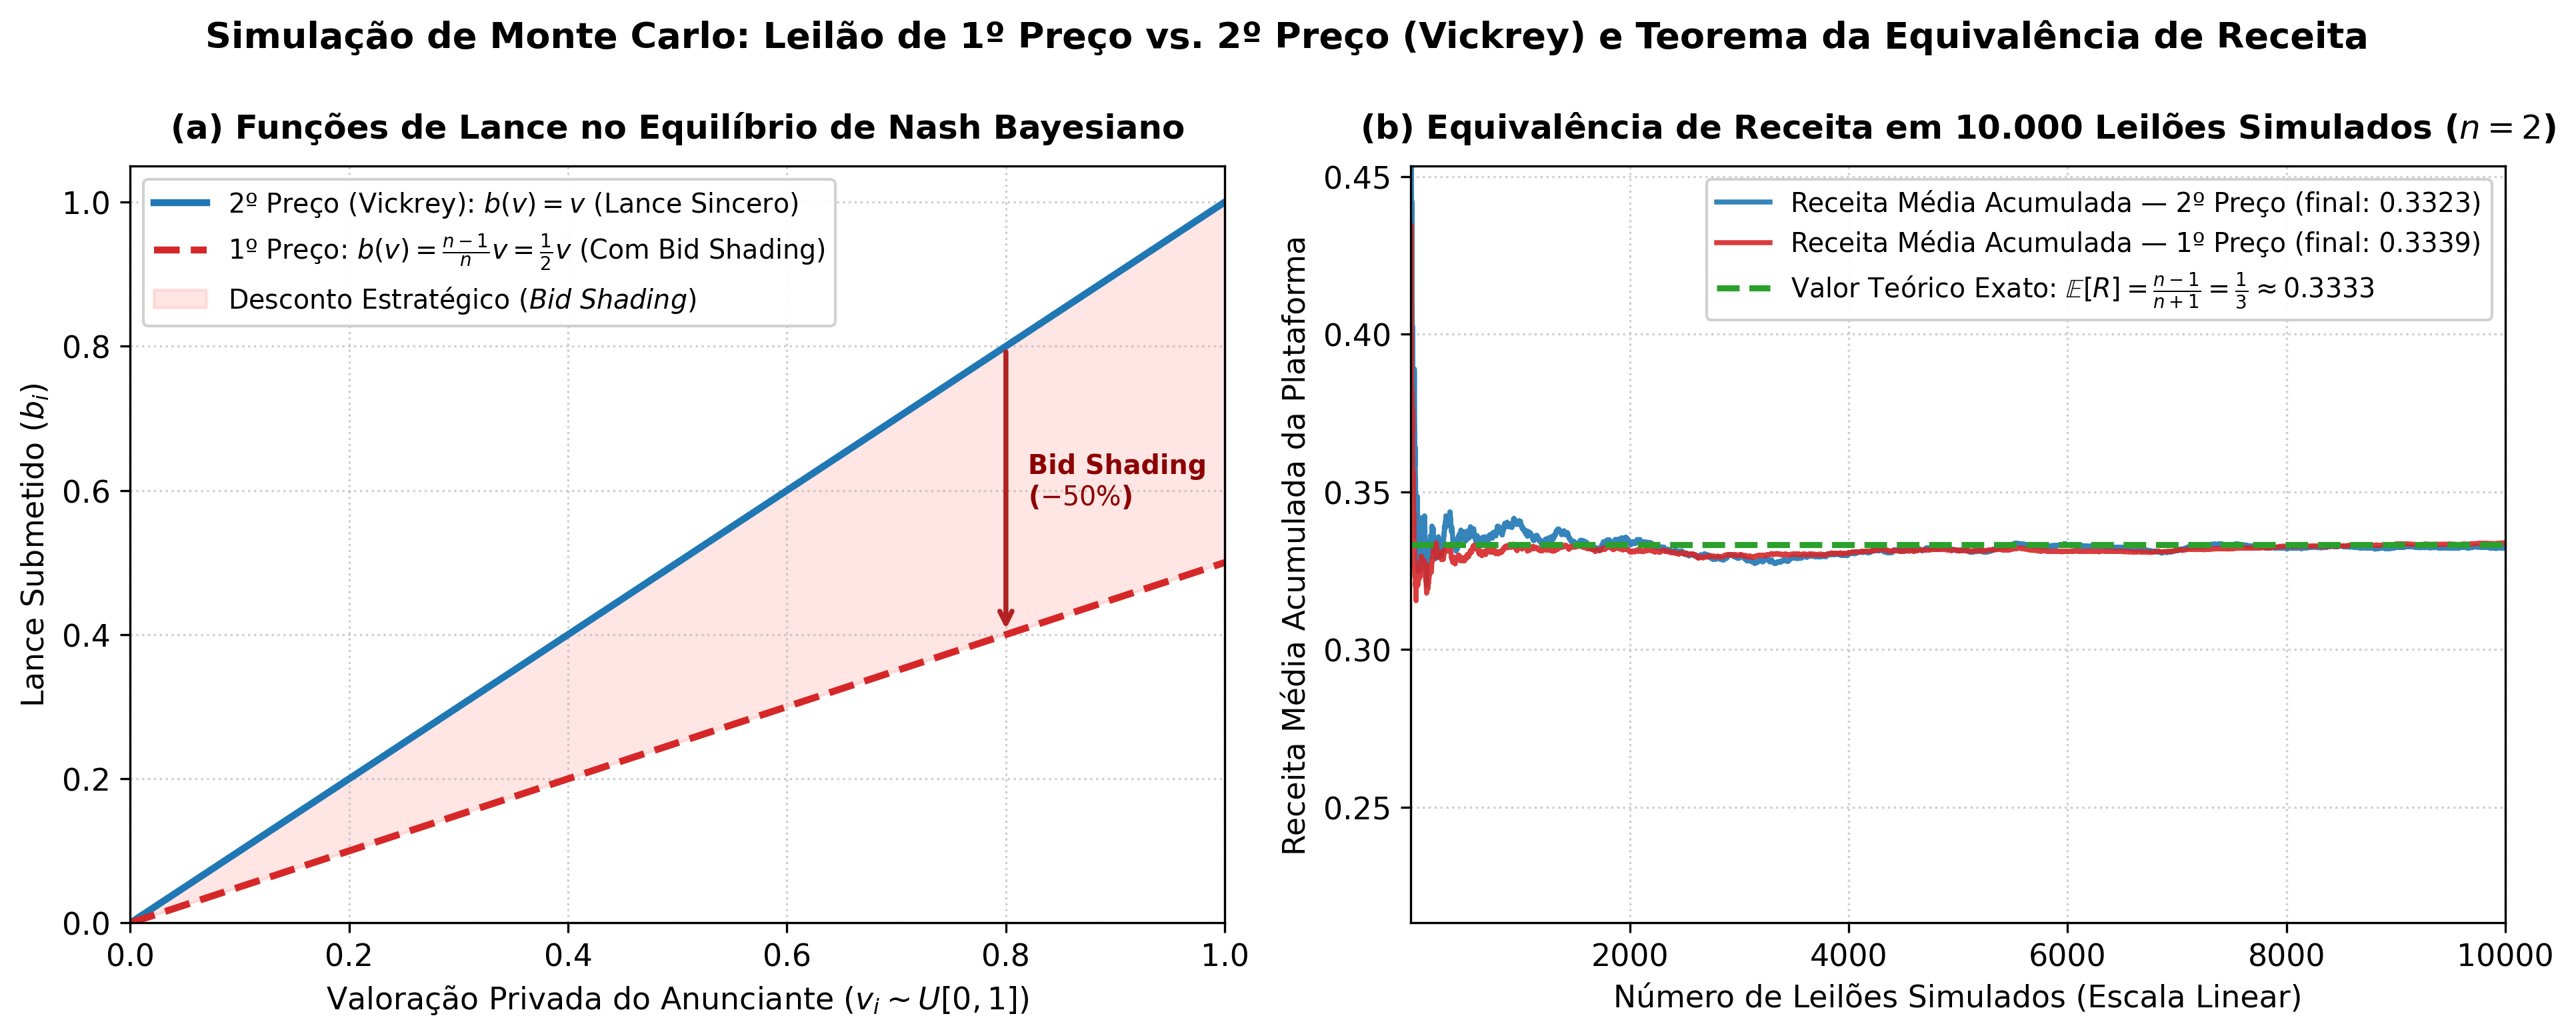
\includegraphics[width=0.75\textwidth]{equivalencia_receita_simulacao.png}
    \par\vspace{0.05cm}
    {\footnotesize Fonte: Elaborado pelos autores (2026).}
    \label{fig:equivalencia_receita}
\end{figure}

Quando a Equivalência de Receita \textbf{quebra} no mundo real \cite[p.~18--26]{klemperer2004}? Quando alguma das Hipóteses (1) a (4) é violada:
\begin{enumerate}[label=\arabic*.]
    \item \textbf{Quebra da Hipótese 3 --- Aversão ao Risco:} Se os compradores têm medo de perder o objeto, no \textbf{1º Preço} eles têm receio de dar um desconto grande e perder por pouco, passando a dar lances mais altos (ex.: $70\%$ do valor em vez de $50\%$). No \textbf{2º Preço}, a estratégia dominante continua sendo $b_i = v_i$. Logo, com compradores avessos ao risco, \textbf{o 1º Preço dá mais receita ao vendedor do que o 2º Preço}!
    \item \textbf{Quebra da Hipótese 2 --- Assimetria entre Jogadores:} Imagine que disputam um lote de 5G uma \textbf{Operadora Gigante} (valor sempre entre \textbf{R\$\,80~mi e R\$\,100~mi}) e uma \textbf{Operadora Pequena} (valor entre \textbf{R\$\,10~mi e R\$\,75~mi}). No \textbf{Leilão Inglês / 2º Preço}, como cada um vai até $100\%$ do seu valor, a Gigante sempre cobrirá a Pequena ($80 > 75$); sabendo que tem $0\%$ de chance de vencer, a Pequena nem se inscreve e a Gigante leva o lote sozinha pelo preço mínimo! Já no \textbf{1º Preço em Envelope Fechado}, a Gigante (digamos, com valor de R\$\,85~mi) sabe que a rival é fraca e coloca só \textbf{R\$\,50~mi} no envelope para lucrar alto, enquanto a Pequena (que tirou R\$\,70~mi) reduz sua margem e coloca \textbf{R\$\,55~mi}. Isso gera um resultado duplo no 1º Preço: (a) a Pequena tem chance real de vencer ($\text{R\$\,55~mi} > \text{R\$\,50~mi}$), atraindo participantes e aumentando a receita; mas (b) quebra-se a \textbf{Hipótese 4a (Alocação Eficiente)}, pois às vezes a Pequena (valor de R\$\,70~mi) vence a Gigante (valor de R\$\,85~mi)!
    \item \textbf{Conluio / Cartel:} Leilões abertos (inglês) e de 2º preço facilitam que membros de um cartel vigiem e punam na hora quem furar o acordo; já o envelope fechado de 1º preço incentiva a ``traição'' do cartel, gerando maior receita para o leiloeiro.
\end{enumerate}

% =============================================================================
\subsection{Maldição do Vencedor (\textit{Winner's Curse})}
\label{subsec:maldicao_vencedor}

Saindo de Valores Privados e entrando em \textbf{Valor Comum} (Definição~\ref{def:cv}), surge a famosa armadilha informacional:

\begin{definicao}[Maldição do Vencedor --- \textit{Winner's Curse}]
\label{def:maldicao_vencedor}
Em um leilão de \textbf{Valor Comum}, suponha que todos os participantes têm estimativas não-viesadas do valor real $V$ (na média, a estimativa de todos acerta $V$, mas uns erram para mais e outros para menos). Se todos usam a mesma regra de dar lance proporcional à sua estimativa, \textbf{quem ganha o leilão não é quem fez a estimativa mais precisa, mas sim quem cometeu o maior erro de superestimação (o mais otimista da sala)!} Se os jogadores não descontarem esse viés ao calcular seus lances, o vencedor frequentemente pagará mais do que o objeto realmente vale ($p > V$) e terá prejuízo \cite[p.~14]{klemperer2004}.
\end{definicao}

Para visualizar isso, \cite[p.~14 e 53]{klemperer2004} usa a analogia do \textbf{pote de moedas}: imagine um pote de vidro com exatamente \textbf{R\$\,100,00} ($V = 100$) leiloado entre 20 alunos. Na média a turma chuta bem (R\$\,100): uns chutam R\$\,70, outros R\$\,95, outros R\$\,105, e o aluno mais otimista da sala chuta \textbf{R\$\,150}. Se cada um der um lance próximo ao que chutou, quem ganha o leilão é justamente o aluno que achou que tinha R\$\,150; mesmo que ele dê um pequeno desconto e pague R\$\,130, ao abrir o pote descobrirá que só havia R\$\,100 e perderá R\$\,30!

Como um jogador racional evita a Maldição do Vencedor no Equilíbrio de Nash Bayesiano? Aplicando o \textbf{Condicionamento na Vitória}: em vez de perguntar \textit{``quanto vale o poço dado que meu geólogo disse 150 milhões?''}, ele pergunta: \textit{``quanto vale o poço dado que meu geólogo disse 150 milhões \textbf{E os geólogos de todas as outras 9 empresas disseram menos que 150 milhões}?''} ($\mathbb{E}[V \mid s_i, \max_{j \neq i} s_j < s_i]$). Por isso, quanto maior o número de concorrentes num leilão de valor comum, mais conservador (menor) deve ser o lance!
